\section{Algorithmes}
    \subsection{Voyageur de commerce}
        \subsubsection{Génération des données}
            La génération des données se fait en deux temps :
            \begin{enumerate}
                \item Génération de points à des coordonnées aléatoires
                \item Génération de la matrice des distances
            \end{enumerate}
        \subsubsection{Interface}
            L'utilisateur sélectionne les points par simple clic,
            et peut annuler ses actions par clic droit.
            A chaque point sélectionné, le programme
            affiche la distance totale entre les points reliés.
            Dès lors qu'un point a été sélectionné, le programme
            affiche la distance minimum calculée, à coté de
            la distance actuelle parcourue par l'utilisateur.
            Lorsque tout les points ont été reliés entre eux,
            le programme raccorde automatiquement le premier
            et le dernier point, afin de former une boucle.
        \subsubsection{Résolution}
            Lors de la sélection du premier point,
            le programme calcule à l'aide de l'algorithme
            du \emph{plus proche voisin} le chemin le plus court.
            Une fois que l'utilisateur a relié tout les points
            entre eux, le programme affiche la solution calculée
            en surimpression de celle proposée par l'utilisateur.
        \subsubsection{Algorithme}
        \begin{lstlisting}
computed_path = [self.matrix[0][ligne]]
self.matrix[0][ligne].visite = vrai
tmp = -1
max_distance = sqrt((max_x - min_x)^2 + (max_y - min_y)^2)
pour i de 1 a matrix[0][0] + 1
    minimum = max_distance
    pour j de 1 a matrix[0][0] + 1
        si 0 < matrix[ligne][j] < minimum
            si matrix[ligne][j].visite = faux
                minimum = matrix[ligne][j]
                tmp = j
            finsi
        finsi
    finpour
    si minimum != max_distance
        computed_path = computed_path + matrix[0][tmp]
        matrix[0][tmp].visite = vrai
        computed_len = computed_len + minimum
        ligne = tmp
    finsi
finpour
comuted_len = computed_len + matrix[1][tmp]
        \end{lstlisting}


	\subsection{Couplage}
		\paragraph{Contexte}
			Le problème du couplage est modélisé par un jeu de choix.
			Il y a plusieurs clients, avec leurs préférences qui ont
			 le choix entre plusieurs pizzas, et le joueur doit
			 satisfaire un maximum de clients.
		\paragraph{Moteur}
			Au demarrage de l'application, le nombre de pizzas et
			 de clients est généré aléatoirement, dans un intervalle
			 assez bas, par soucis de complexité.
			Les préférences de chaque client sont aussi générées aléatoirement,
			 mais dans l'optique qu'un client ait au minimum une préférence.
		\paragraph{Interface}
		    L'écran est divisé en trois colonnes :
		    \begin{itemize}
		        \item[à gauche] les préférences de chacun des clients
		        \item[au centre] les clients
		        \item[à droite] les pizzas disponibles
		    \end{itemize}

		L'utilisateur \emph{sélectionne} un client en cliquant dessus.
		    Une fois un client sélectionné, il est possible
		    d'associer une pizza à ce client, en cliquant dessus.
		    Si la pizza est déjà attribuée, ou si le client a déjà
		    une pizza qui lui est affectée, un message d'erreur s'affiche.
		    Si ni le client n'a de pizza, ni la pizza de client, l'association
		    se fait et est représentée par un trait.
		L'utilisateur a la possibilité d'annuler ses choix en cliquant avec le bouton
		    droit de la souris (ce qui annule la dernière action).
		\paragraph{Résolution}
			L'algorithme permet d'avoir la solution comportant un maximum de clients
			 satisfaits et de vérifier si la solution proposée par le joueur correspond
			 à la meilleure solution possible.
 			Si l'utilisateur n'a pas trouvé la solution optimale, la solution s'affiche
			 en surimpression sur le choix du joueur.
            

		\paragraph{Algorithme de résolution}
			Pour résoudre ce problème il faut dans un premier temps le modéliser.
            Pour cela, nous introduisons un nouveau problème standard qui est celui du flot maximal sur un
            réseau. Pour trouver le flot maximale qui parcoura ce graphe on utilisera l'algorithme de flot
             maximum de Ford-Fulkerson.

        \paragraph{Définition d’un flot sur un graphe}

	    Dans la théorie des graphes, un réseau à flot est un graphe directe ou chaque arc à une capacité et un flot, il va d'un sommet dit source à un sommet puit. 
	    La valeur du flot sur l'arc ne peut pas dépasser la capacité de l'arc. Un flot doit respecter la condition que la valeur d'un flot entrant dans un arc 
	    est égale à la valeur de flot qui sort de cet arc hormis la source et le puit. Un tel réseau peut être utilisé pour modeliser un traffic routier, des canalisations d'eau,
	    le courant électrique dans un circuit ...
	    Il s'agit là de la \emph{loi des noeuds} de Gustav Kirchhoff, physicien allemand de la fin du XIX\up{ème} siècle:


\begin{quotation}
 	    En chaque point du réseau électrique, la somme des intensités entrantes est égale à la somme des intensités sortantes.

\end{quotation}
\begin{figure}[h]
\begin{center}
    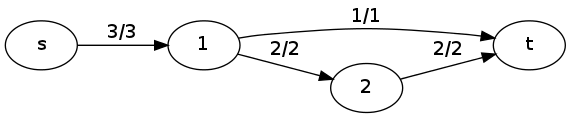
\includegraphics[width=.8\textwidth]{flow.png} 
    \caption{Exemple illustrant la notion de flot}

\end{center}
\end{figure}

      \paragraph{modelisation du graphe correspondant au problème de couplage}
      La source est liée à toute les fourmis par un arc de capacité égale à 1, en effet, un client ne peut pas choisir plusieurs pizza.
      Ensuite chaque pizza est reliée au puit par un arc de capacité 1, chaque pizza ne peut être sélectionner qu'une seule fois.
      Ensuite pour définir les préférence de chaque client, on relie le client au pizza qu'il aime avec un arc de capacité supérieur à 1.

\begin{figure}[h]
\begin{center}
    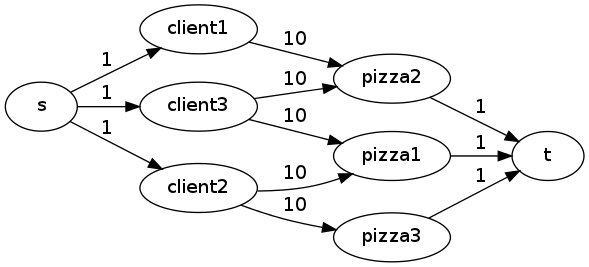
\includegraphics[width=.8\textwidth]{exemple_couplage.png}
    \caption{Exemple illustrant la notion de flot}

\end{center}
\end{figure}

Ici on à trois client et trois pizzas disponibles. Le client 1 n'aime que la pizza 1, le client 2 aime la pizza 1 et la pizza 3 et le client 3 n'aime que la pizza 1 et la pizza 2.


\paragraph{algorithme de Ford-Fulkerson}


    \subsection{Sac à Dos}
        \paragraph{Contexte}
        On pourra modéliser ce problème par un tableau contenant les objets et leur
        valeur en vis-à-vis. L'utilisateur fera glisser les objets du tableau vers
        le sac à dos. Un indicateur permettra de visualiser le poids actuel total
        des objets dans le sac, le poids maximal que peut supporter le sac, et le
        poids restant (différence entre ces deux résultats).

            Dans ce mini-jeu, le but du joueur est d'aider un pizzaiolo à
            sélectionner des ingrédients à transporter à un concours de pizza.
            Il ne peut pas prendre tout ce qu'il souhaite et doit faire des
            choix entre qualité et quantité : de bons ingrédients lui donneront
            plus de points par le jury, cependant la pizza présentée a un poids
            limité au gramme près.
        \paragraph{Moteur}
            Au démarrage de l'application, une liste d'ingrédients est créée.
            Pour respecter une certaine logique, on ne peut pas générer des
            chiffres aléatoirement. (Il semblerait assez illogique qu'une
            garniture au fromage pèse plusieurs centaines de grammes par
            exemple.)
        \paragraph{Interface}
            L'interface se présente en 2 colonnes. La première, à gauche,
            contient les objets disponibles pour la pizza. La seconde, à droite,
            montre le contenu actuel de la pizza que le joueur a choisi.
            Un clic sur l'icone d'un ingrédient permet de l'échanger entre
            les deux colonnes.
            Lorsque l'utilisateur a terminé, il clique sur le bouton de
            validation pour savoir s'il a trouvé la solution correcte.
        \paragraph{Résolution}
            La résolution du problème s'effectue grâce à un calcul de la solution optimale
            par programmation dynamique. Notons $V(k,y)$ la valeur optimale au problème du sac à dos
            réduit au $k$ premier objet avec un sac de poids maximal de $y$.
            $y_{k}$ le poids de l'objet k et $v_{k}$ la valeur de l'objet $k$.

            Si $ y - y_{k} >= 0 $

                $V(k,y) = max\{ V(k-1,y)  ,v_{k} + V(k-1,y-y_{k}) \}$

            Sinon

                $V(k,y) = V(k-1,y)$

            On notera aussi que si il n'y a pas d'objet on a : $V(0,y) = 0$
            De plus si le poids est nul on a: $V(k,0) = 0$

	\emph{Algorithme}

\begin{lstlisting}
solution = []
pour i allant de 0 a nombre_Objet+ 1
    pour j allant de 0 a poids_maximum + 1
        si i != 0 et j != 0
            w = Objet[i].poids
            si j > w alors
                si solution[i-1][j].poids > Objet[i].valeur+
                            ...solution[i-1][j-w].valeur
                    solution[i][j] = solution[i-1][j]
                sinon
                    solution[i][j] = solution[i-1][j-w] + Objet[i]
                finsi
            sinon
                solution[i][j] = solution[i-1]
            finsi
        sinon
            solution[i][j] = 0
        finsi
    finpour
finpour
\end{lstlisting}


\subsection{Problème du plus court chemin}

        \paragraph{Contexte}
	    Dans ce mini-jeu vous travaillerez en tant que livreur de pizza. On vous a demandé de 
	    livrer une pizza à l'autre bout de la ville. Pour cela, il vous faudra trouver le plus court chemin
	    pour vous rendre de la pizzeria jusqu'au lieu de la livraison.
        \paragraph{Moteur}
            Au démarrage du jeu, le programme génère un graphe
            représentant des lieux de la ville. Ces lieux sont reliés par des arcs pondérés.
            Le poids des arcs correspond à la distance entre chaque lieu.

        \paragraph{Interface}

        L'utilisateur pourra cliquer sur les différents lieux, tour à tour,
        pour se déplacer. Un compteur kilométrique indiquera la
        distance parcourue en temps réel.

        Le joueur peut effectuer un clic droit pour annuler son dernier
        mouvement.

        Pour revenir au début il suffit de cliquer sur la ville de départ.

        Le jeu continue tant que le joueur n'a pas trouvé le chemin
        le plus court. Il peut aussi cliquer sur \og solution\fg, qui
        affichera le chemin segment par segment.

\begin{figure}[h]
\begin{center}
    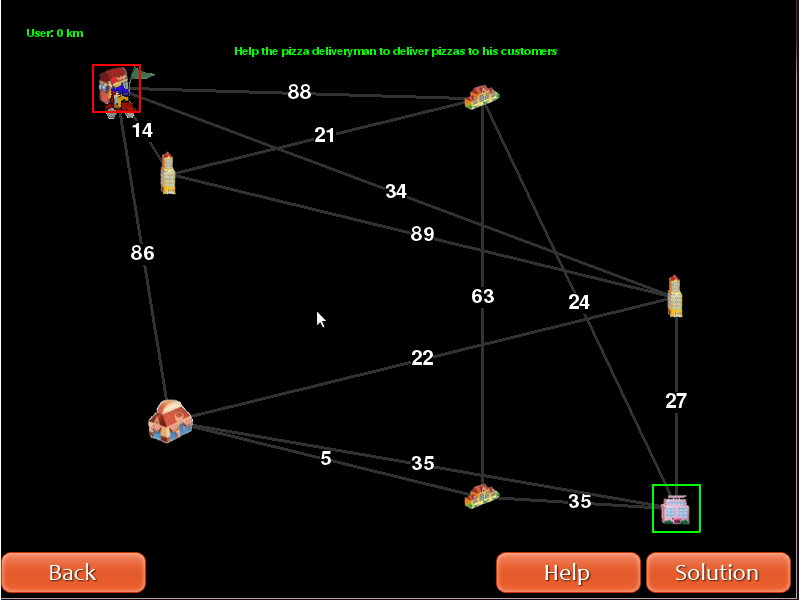
\includegraphics[width=.8\textwidth]{plus_court_1.png} 
    \caption{Interface pour le problème du plus court chemin}
\end{center}
\end{figure}

        \paragraph{Résolution}
            Lorsque la ville de début et la ville finale sont reliées,
            on appelle la méthode de résolution par l'algorithme de \emph{Dijkstra}.

            Le programme affiche ensuite si le joueur à trouvé la solution optimale.

		\paragraph{Algorithme de Dijkstra} ~

			L'algorithme de Dijkstra est l'un des algorithmes de résolution du problème du
			\emph{plus court chemin} les plus connus. Cet algorithme s'applique à des graphes pondérés orientés ou non.

			L'algorithme de \emph{Dijkstra} :
			\begin{lstlisting}
liste_sommets = [+oo pour i dans sommets]
S(liste_sommets[0]) = 0
tantque taille(liste_sommets) != 0
    element_courant = min(liste_sommets)
    mettre_a_jour(element_courant)
    supprimer element_courant de liste_sommets
fintantque
			\end{lstlisting}
			Pour mettre à jour un sommet i:

				Pour chaque autre sommet j qui est relié à ce sommet i on vérifie si
				la valeur de j est supérieure à la valeur de i plus la valeur de l'arc entre i et j.

			\begin{lstlisting}
mettre_a_jour(sommet):
pour chaque sommet_choisit dans graphe
    si sommet_choisit.visiter == faux
        si sommet_choisit.valeur > sommet.valeur + ...
            ... distance entre les deux sommets
		    sommet_choisit.valeur = sommet.valeur + ...
            ... distance entre les deux sommets
        finsi
	finsi
finpour
			\end{lstlisting}


Présentation de l'Algorithme de \emph{Dijkstra} par un exemple:
\begin{figure}[h]
\begin{center}
    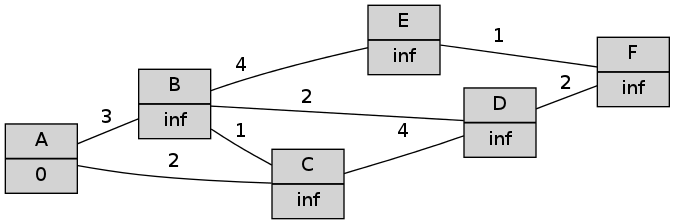
\includegraphics[width=.8\textwidth]{dot1.png} 
    \caption{Graphe connexe non orienté et pondéré}

\end{center}
\end{figure}

\begin{figure}[h]
\begin{center}
    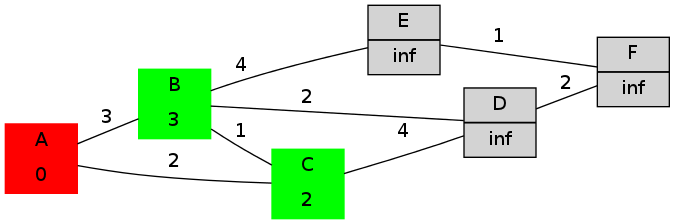
\includegraphics[width=.8\textwidth]{dot2.png} 
    \caption{Étape 1 : à partir de la ville A, 2 villes sont accessibles, B et C qui se voient donc affecter des poids respectifs de 3 et 2 tandis que les autres villes sont affectées d'une distance infinie.}
\end{center}
\end{figure}

\begin{figure}[h]
\begin{center}
    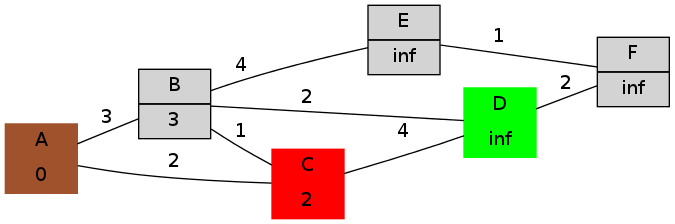
\includegraphics[width=.8\textwidth]{dot3.png} 
    \caption{Étape 2 : On choisit de mettre à jour les villes voisines du point C, car c'est lui qui possède la plus petite valeur. Depuis C on a accès à deux point B et D mais on met seulement D à jour car le chemin de A à B en passant par C n'est pas inférieur au chemin de A à B.}
\end{center}
\end{figure}

\begin{figure}[h]
\begin{center}
    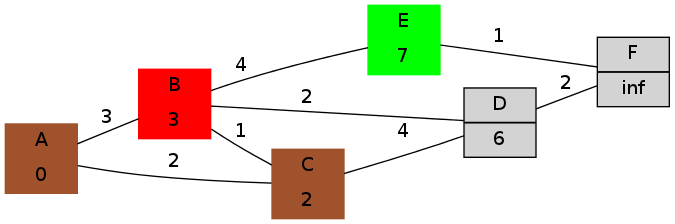
\includegraphics[width=.8\textwidth]{dot4.png} 
    \caption{Étape 3 : On choisit de mettre à jour les villes voisines du point B, car c'est lui qui possède la plus petite valeur. Depuis B on a accès au point E.}
\end{center}
\end{figure}

\begin{figure}[h]
\begin{center}
    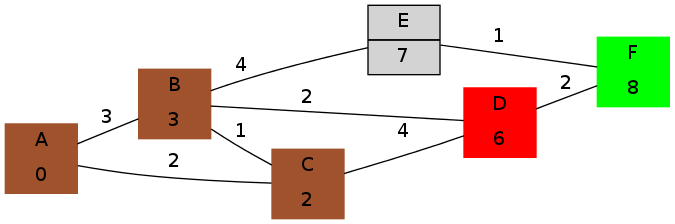
\includegraphics[width=.8\textwidth]{dot5.png} 
    \caption{Étape 4 : On choisi de mettre à jour les villes voisines du point D.}
\end{center}
\end{figure}

\begin{figure}[h]
\begin{center}
    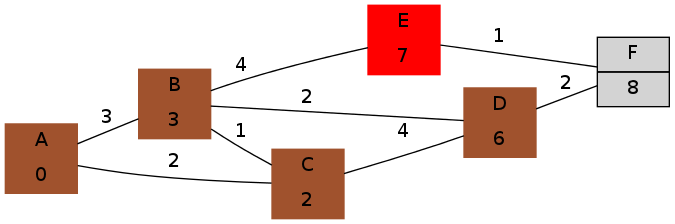
\includegraphics[width=.8\textwidth]{dot6.png} 
    \caption{Étape 5 : On choisit de mettre à jour les villes voisines du point E.}
\end{center}
\end{figure}


\begin{figure}[h]
\begin{center}
    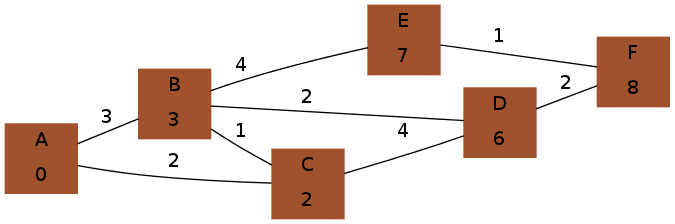
\includegraphics[width=.8\textwidth]{dot7.png} 
    \caption{Pour aller du point A au point F, la distance la plus courte et de 8.}
\end{center}
\end{figure}
